
Dire~\cite{Hoche:2015sya}.  PFN~\cite{Komiske:2018cqr}.

Here, we will discuss now useless triple-collinear corrections to Dire were, and
how awesome double-soft contributions are.

\dots some Dire bullet points
\begin{itemize}
\item parton showers serve two purposes: $1)$ the distribution of low-multiplicity
(hard-scattering) states over states of arbitrarily high multiplicity, as well
as $2)$ generating the effect of resummation for observable depending only on 
low-multiplicity configurations.
\item these two purposes are often in conflict, e.g.\ choices to improve
$2)$ often limit the potential to improve $1)$ -- and vice versa. these
conflicts are not apparent at lowest (i.e.\ leading) order.
\item parton showers typically include states distributed with leading-order 
(leading-logarithmic) rate in their emission- and no-emission probabilities.
\item the rate of subsequent splittings is independent of the rate of
previous splittings, and the evolution scales at which splittings occur is
successively ordered -- such that resummation can occur.
\item with demand for more precise event generation, improved parton showers
are necessary. For example, the use of NLO PDFs (as e.g.\ mandated in NLO+PS
matching) in the parton shower in principle requires parton showers beyond
lowest order.
\item one way to improve the all-order behavior of the parton shower (point $2)$ 
above) while preserving a systematically improvable state distribution (point $1)$ 
above) is to consistently include higher-order and higher-multiplicity 
splitting functions in the parton shower.
\item
\item \emph{more to come, taking a break\dots}
\end{itemize}

\begin{figure}[h!]
\subfigure[blub]{
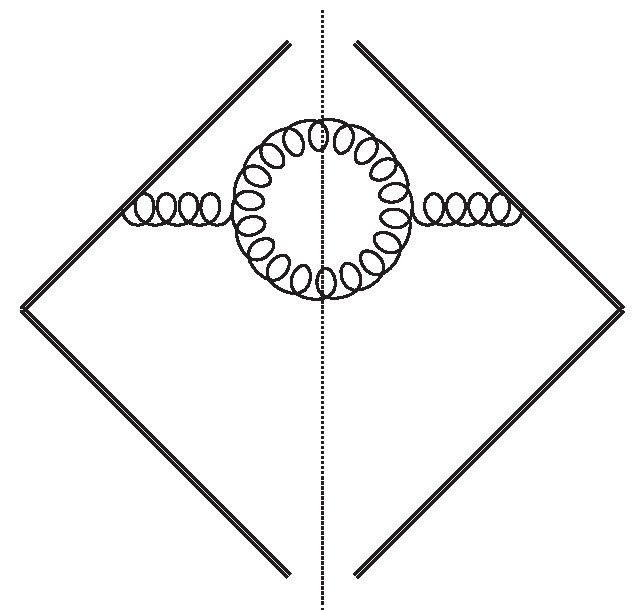
\includegraphics[width=0.23\textwidth]{figs/nlo_real_vpcg.pdf}
\label{fig:jets:np:triplecollineardiagrams2}
}
\subfigure[blub]{
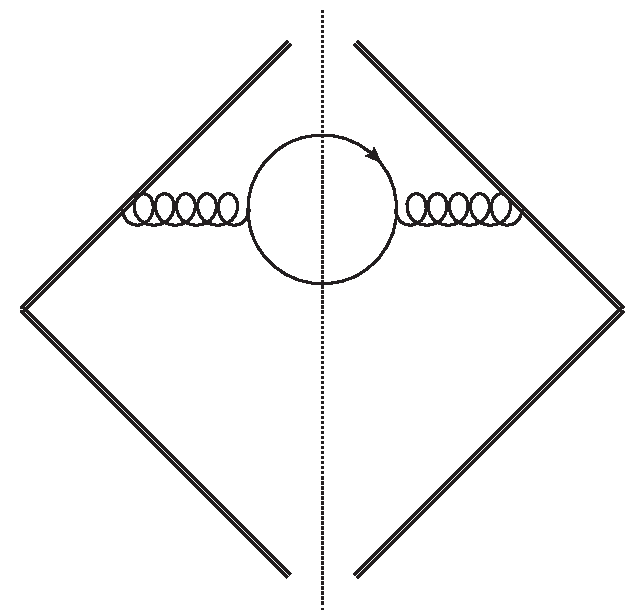
\includegraphics[width=0.23\textwidth]{figs/nlo_real_vpcq.pdf}
\label{fig:jets:np:triplecollineardiagrams2}
}
\subfigure[blub]{
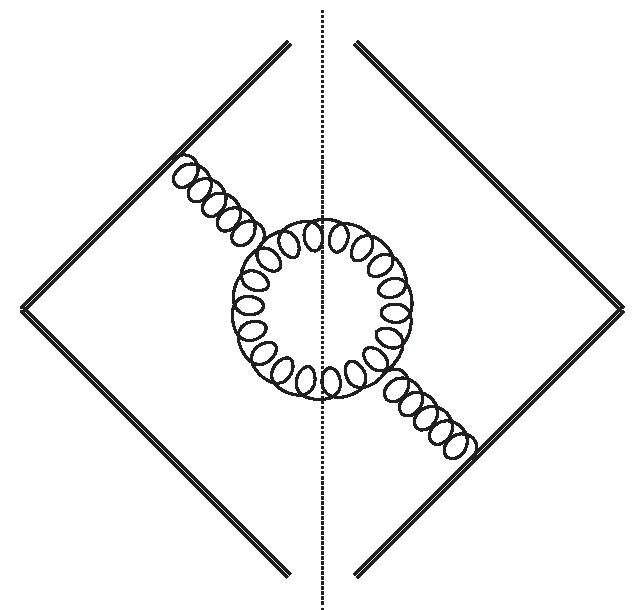
\includegraphics[width=0.23\textwidth]{figs/nlo_real_vpsg.pdf}
\label{fig:jets:np:triplecollineardiagrams2}
}
\subfigure[blub]{
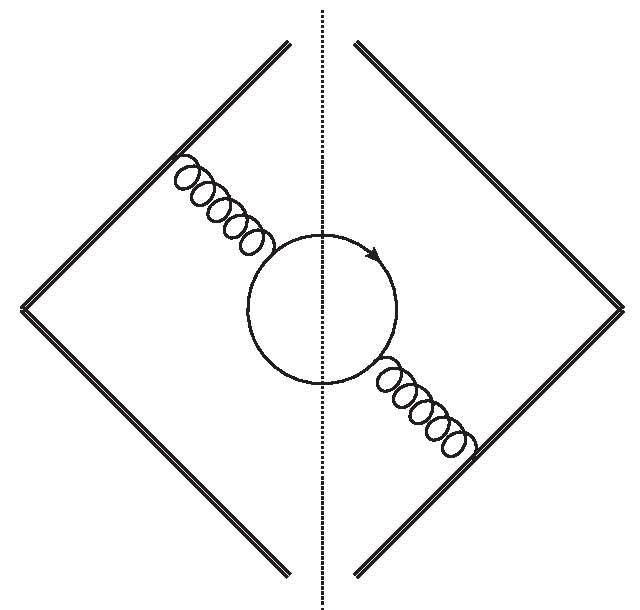
\includegraphics[width=0.23\textwidth]{figs/nlo_real_vpsq.pdf}
\label{fig:jets:np:triplecollineardiagrams2}
}
\\
\subfigure[blub]{
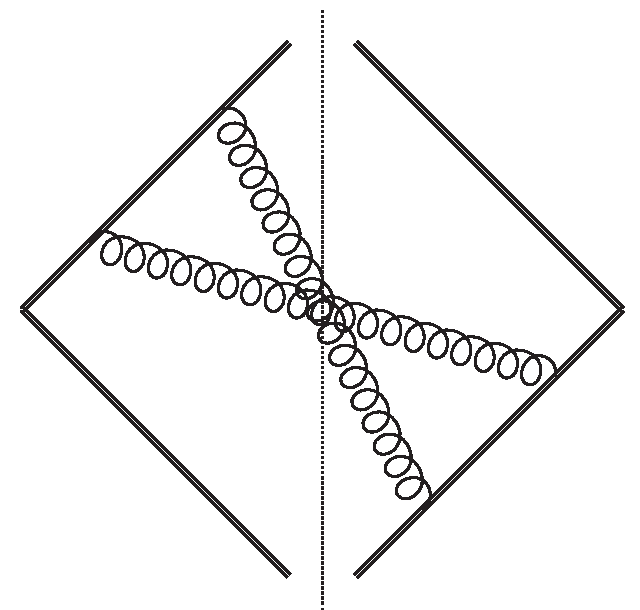
\includegraphics[width=0.23\textwidth]{figs/nlo_real_box1.pdf}
\label{fig:jets:np:triplecollineardiagrams1}
}
\subfigure[blub]{
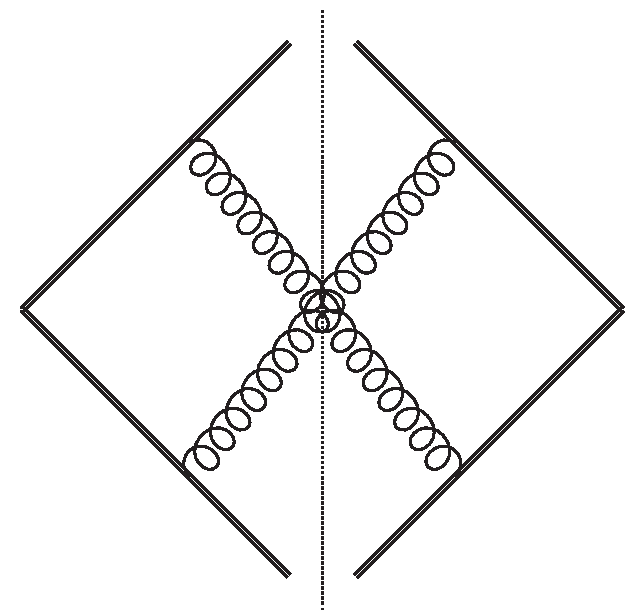
\includegraphics[width=0.23\textwidth]{figs/nlo_real_box2.pdf}
\label{fig:jets:np:triplecollineardiagrams2}
}
\subfigure[blub]{
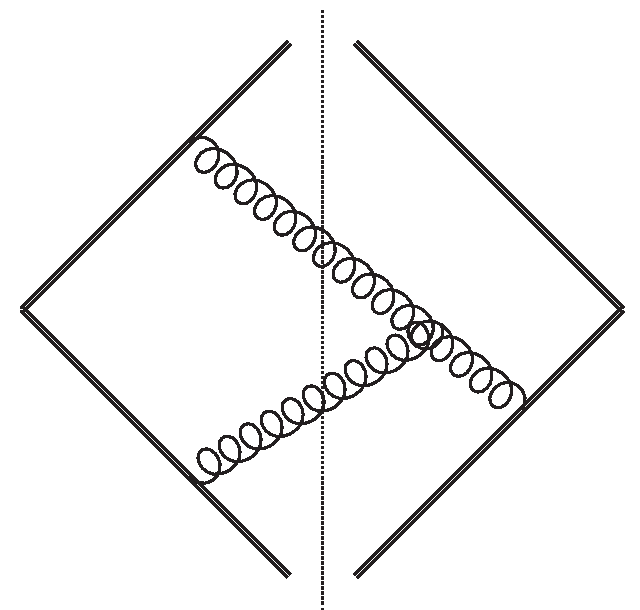
\includegraphics[width=0.23\textwidth]{figs/nlo_real_tgc1.pdf}
\label{fig:jets:np:triplecollineardiagrams2}
}
\subfigure[blub]{
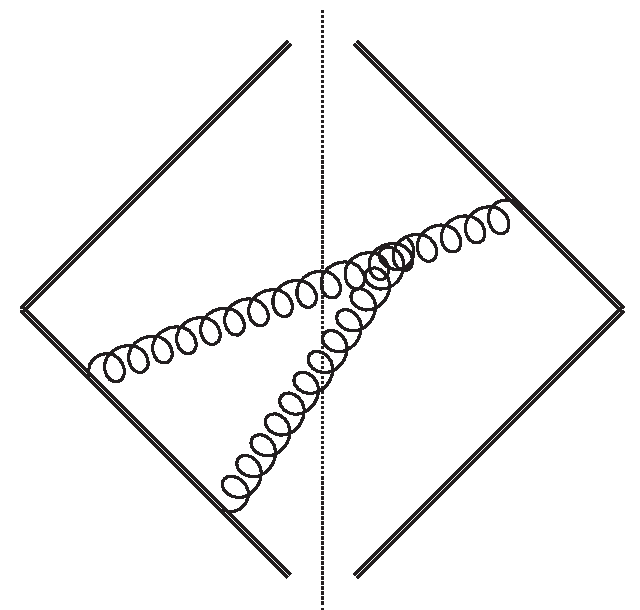
\includegraphics[width=0.23\textwidth]{figs/nlo_real_tgc2.pdf}
\label{fig:jets:np:triplecollineardiagrams2}
}
\caption{Replace me with proper diagrams!}
\label{fig:jets:np:triplecollineardiagrams}
\end{figure}

\begin{figure}[h!]
\centering
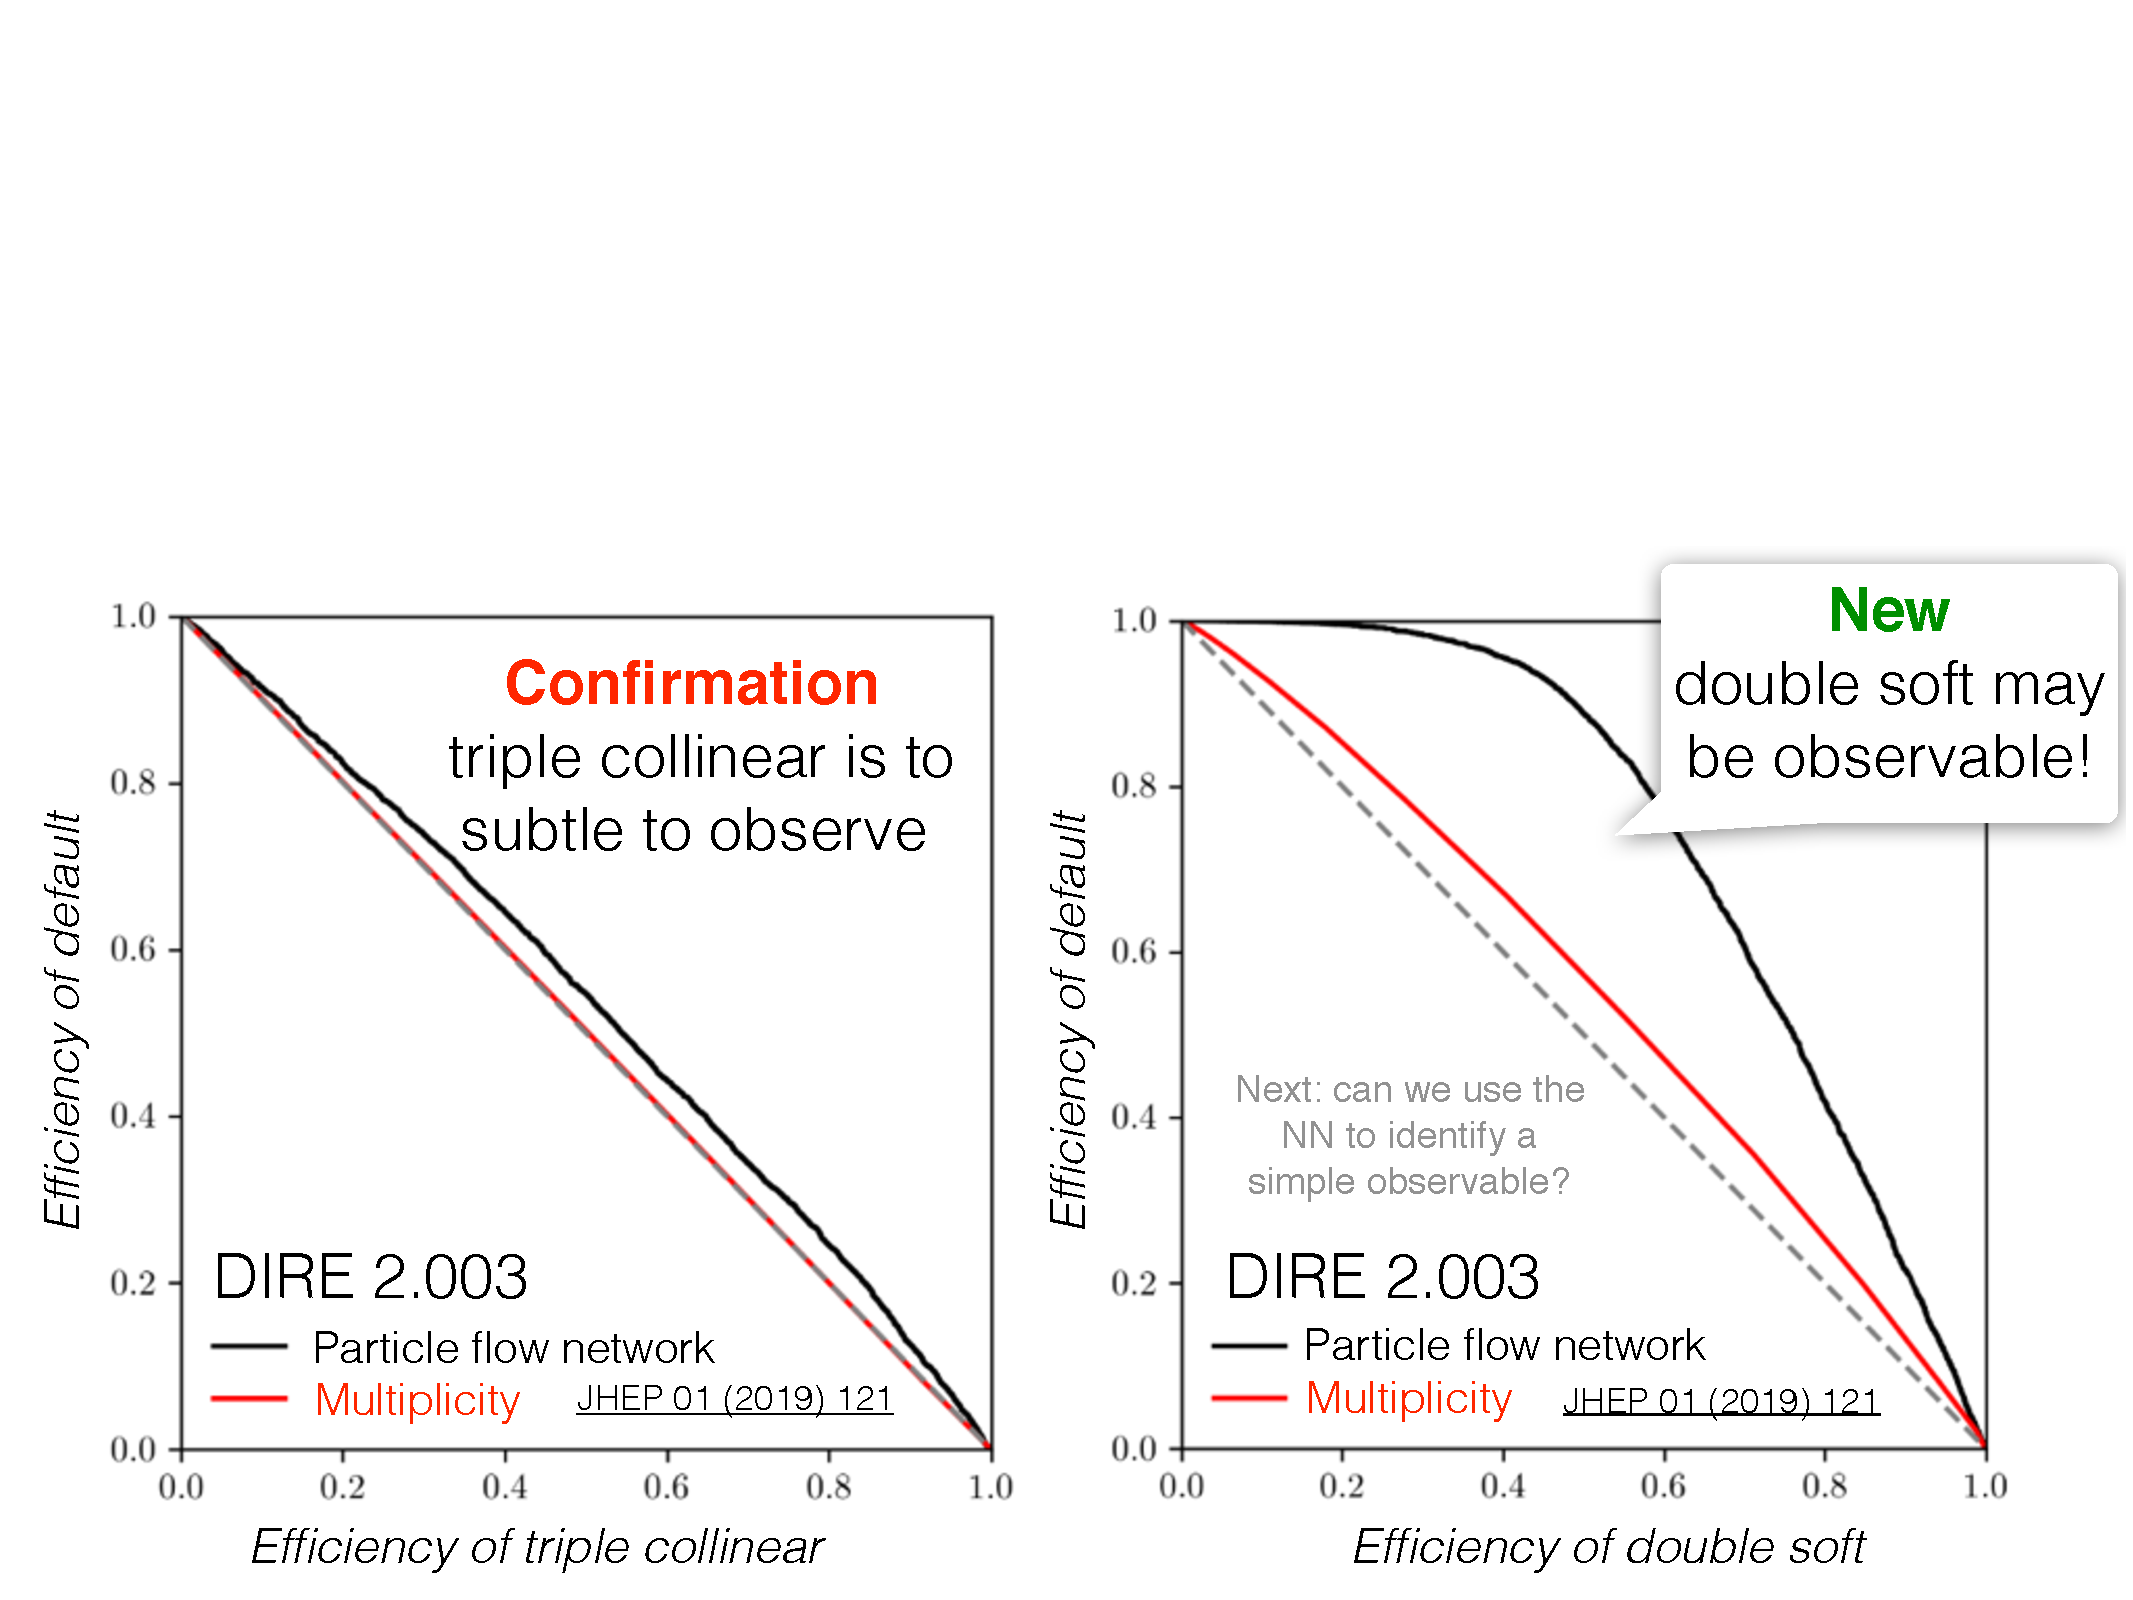
\includegraphics[width=0.85\textwidth]{figs/triplecollinear.pdf}
\caption{Replace me with proper plots!}
\label{fig:jets:np:triplecollinearNN}
\end{figure}




